\documentclass[spanish,letterpaper,oneside]{article}

\def\documenttitle {Aplicaciones del álgebra lineal}
\def\documentsubtitle {Actividad 1, Fase 1: mapa cognitivo de telaraña}
\def\documentsubject {Actividad 1 - Álgebra Lineal}
\def\documentauthor {Equipo de Álgebra Lineal}
\def\coursename {Álgebra Lineal}
\def\coursecode {Fase 1}
\def\universityname {Universidad Autónoma de Nuevo León}
\def\universityfaculty {Facultad de Agronomía}
\def\universitydepartment {Ingeniero Agrónomo}
\def\universitydepartmentimage {UANL/assets-uanl/logo-uanl.png}
\def\universitydepartmentimagecfg {width=3.2cm}
\def\universitylocation {General Escobedo, Nuevo León, México}
\def\authortable {
  \begin{tabular}{ll}
    \textbf{Modalidad:} & Equipo de 2 a 3 estudiantes \\
    Programa: & Ingeniero Agrónomo \\
    Unidad de aprendizaje: & \coursename \\
    Evidencia: & Mapa cognitivo de telaraña \\
    Fase: & 1 \\
    & \\
    \multicolumn{2}{l}{Fecha de realización: \today} \\
    \multicolumn{2}{l}{\universitylocation}
  \end{tabular}
}

\input{template}
\usepackage{pdflscape}
\usepackage{tikz}
\usetikzlibrary{calc,positioning,shapes.geometric}

\definecolor{agrogreen}{RGB}{39,105,74}
\definecolor{agrolight}{RGB}{221,239,226}
\definecolor{soilbrown}{RGB}{134,91,55}
\definecolor{webblue}{RGB}{42,102,153}
\tikzset{
  webline/.style={draw=agrogreen!58,line width=0.75pt},
  spoke/.style={draw=soilbrown!75,line width=1.05pt},
  center/.style={circle,draw=agrogreen!90,fill=agrogreen,text=white,
    font=\bfseries\small,align=center,minimum size=2.6cm,text width=2.15cm},
  field/.style={rounded corners=4pt,draw=webblue!90,fill=webblue!10,
    font=\bfseries\scriptsize,align=center,text width=2.45cm,inner sep=4pt},
  detail/.style={rounded corners=3pt,draw=agrogreen!85,fill=agrolight,
    font=\scriptsize,align=center,text width=3.05cm,inner sep=4pt}
}

\begin{document}
\templatePortrait
\templatePagecfg
\onehalfspacing

\begin{abstractd}
Vectores, matrices, sistemas lineales, transformaciones, mínimos cuadrados y valores propios relacionan seis ámbitos cotidianos: agricultura de precisión, gráficos digitales, navegación y posicionamiento, buscadores y recomendaciones, imágenes médicas, y economía y planeación. Estas estructuras convierten mediciones y relaciones entre variables en modelos útiles para interpretar información y apoyar decisiones.
\end{abstractd}

\templateIndex
\templateFinalcfg

\section{Introducción}
El álgebra lineal estudia vectores, matrices, transformaciones lineales y sistemas de ecuaciones. Aunque estos conceptos suelen presentarse de forma abstracta, constituyen un lenguaje para organizar datos y describir relaciones entre muchas variables. Las matrices permiten representar información estructurada; los sistemas lineales permiten hallar cantidades desconocidas; y los valores y vectores propios ayudan a reconocer comportamientos dominantes en procesos complejos \citep{lay2021linear,strang2023introduction}.

Estas ideas intervienen en actividades cotidianas y en el trabajo agronómico. Las mediciones de suelo y cultivo, las coordenadas de navegación, los píxeles de una imagen y los flujos de recursos pueden representarse con vectores y matrices. Comparar esos campos permite reconocer una misma lógica: definir variables, expresar sus relaciones y obtener una interpretación útil sin separar el resultado matemático de las condiciones del problema.

\section{Álgebra lineal en contextos cotidianos y agronómicos}
\subsection{Vectores, matrices y relaciones lineales}
Los vectores reúnen magnitudes ordenadas y las matrices organizan conjuntos de observaciones o transformaciones. Los sistemas lineales relacionan variables conocidas y desconocidas; los mínimos cuadrados aproximan soluciones cuando las mediciones contienen variación; y los valores propios describen comportamientos que permanecen dominantes bajo una transformación \citep{meyer2000matrix}. En el mapa, cada rama enlaza un campo, una aplicación concreta y la estructura algebraica que permite estudiarla.

% Técnica didáctica: mapa cognitivo de telaraña con tema central,
% campos en los radios y aplicaciones/objetos algebraicos en la red.
\begin{landscape}
\thispagestyle{empty}
\begin{center}
{\Large\bfseries Mapa cognitivo de telaraña\par}
\vspace{0.15cm}
\begin{adjustbox}{max totalsize={0.94\linewidth}{0.72\textheight},center}
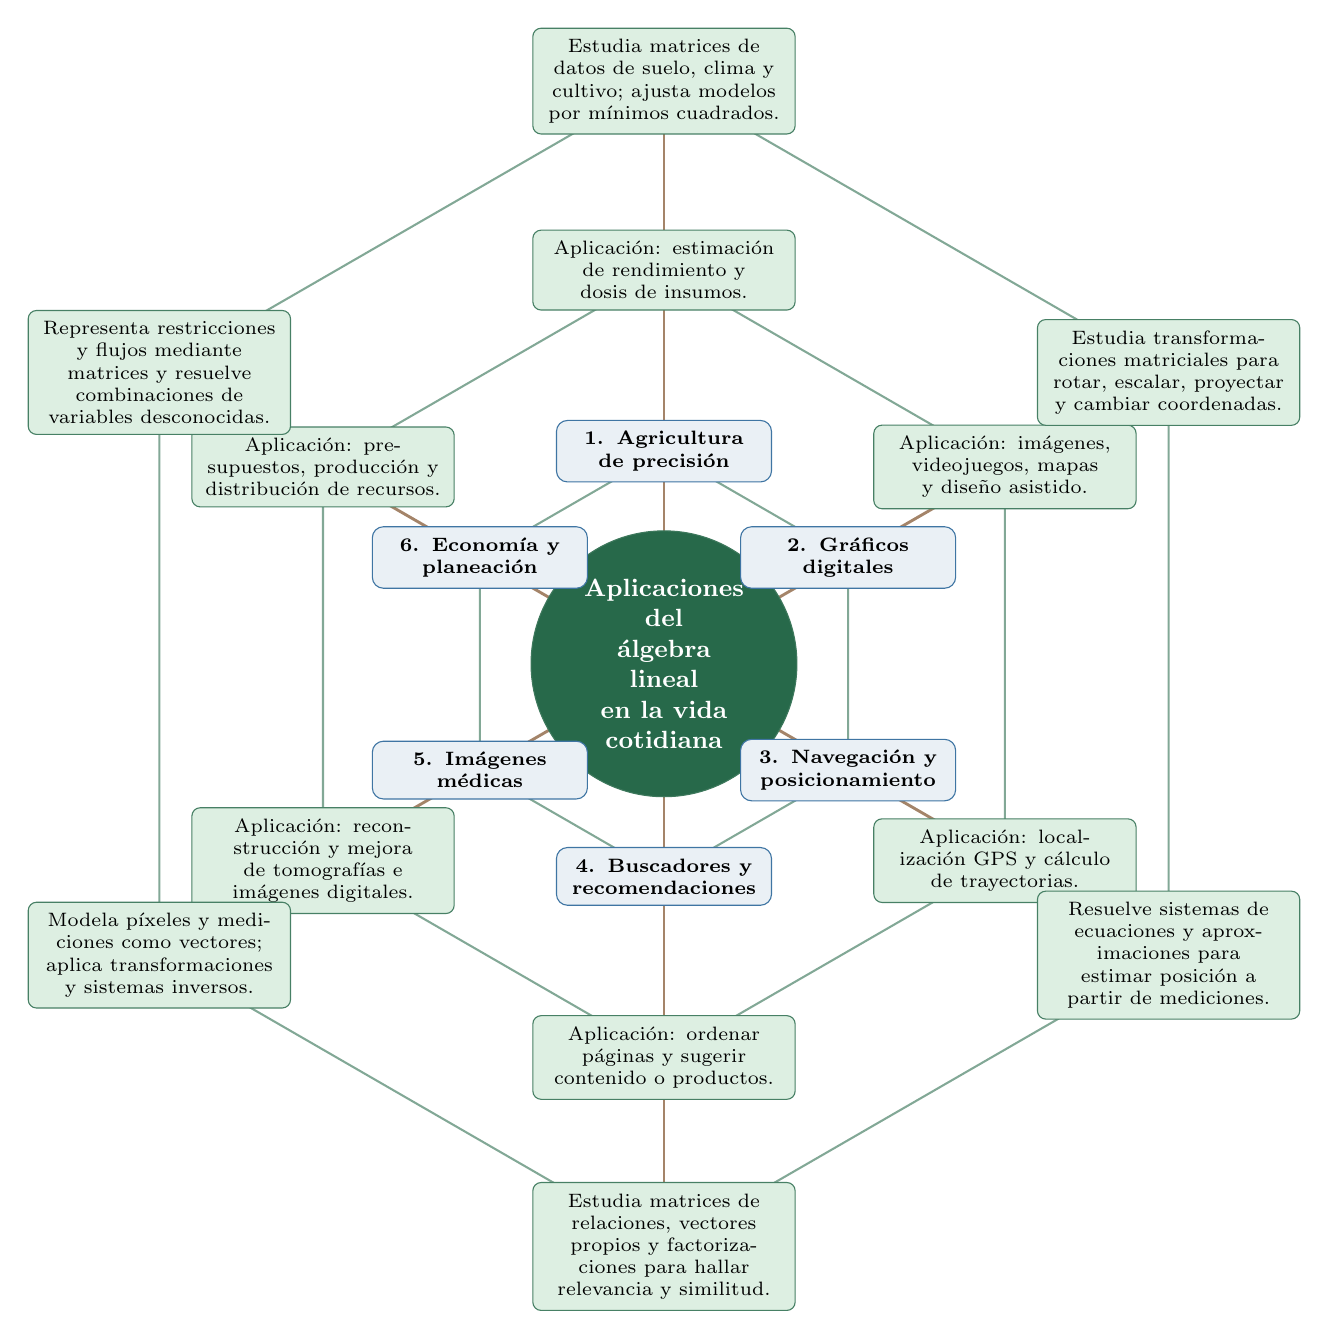
\begin{tikzpicture}[x=1cm,y=1cm]
  % Red compacta de tres niveles hexagonales unidos por radios.
  \foreach \r in {2.7,5.0,7.4}{
    \draw[webline,rounded corners=8pt]
      (90:\r) -- (30:\r) -- (-30:\r) -- (-90:\r) -- (-150:\r) -- (150:\r) -- cycle;
  }
  \foreach \a in {90,30,-30,-90,-150,150}{
    \draw[spoke] (0,0) -- (\a:7.75);
  }

  \node[center] at (0,0) {Aplicaciones del\\álgebra lineal\\en la vida cotidiana};

  \node[field] at (90:2.7) {1. Agricultura\\de precisión};
  \node[detail] at (90:5.0) {Aplicación: estimación de rendimiento y dosis de insumos.};
  \node[detail] at (90:7.4) {Estudia matrices de datos de suelo, clima y cultivo; ajusta modelos por mínimos cuadrados.};

  \node[field] at (30:2.7) {2. Gráficos\\digitales};
  \node[detail] at (30:5.0) {Aplicación: imágenes, videojuegos, mapas y diseño asistido.};
  \node[detail] at (30:7.4) {Estudia transformaciones matriciales para rotar, escalar, proyectar y cambiar coordenadas.};

  \node[field] at (-30:2.7) {3. Navegación y\\posicionamiento};
  \node[detail] at (-30:5.0) {Aplicación: localización GPS y cálculo de trayectorias.};
  \node[detail] at (-30:7.4) {Resuelve sistemas de ecuaciones y aproximaciones para estimar posición a partir de mediciones.};

  \node[field] at (-90:2.7) {4. Buscadores y\\recomendaciones};
  \node[detail] at (-90:5.0) {Aplicación: ordenar páginas y sugerir contenido o productos.};
  \node[detail] at (-90:7.4) {Estudia matrices de relaciones, vectores propios y factorizaciones para hallar relevancia y similitud.};

  \node[field] at (-150:2.7) {5. Imágenes\\médicas};
  \node[detail] at (-150:5.0) {Aplicación: reconstrucción y mejora de tomografías e imágenes digitales.};
  \node[detail] at (-150:7.4) {Modela píxeles y mediciones como vectores; aplica transformaciones y sistemas inversos.};

  \node[field] at (150:2.7) {6. Economía y\\planeación};
  \node[detail] at (150:5.0) {Aplicación: presupuestos, producción y distribución de recursos.};
  \node[detail] at (150:7.4) {Representa restricciones y flujos mediante matrices y resuelve combinaciones de variables desconocidas.};
\end{tikzpicture}
\end{adjustbox}
\vspace{0.1cm}

\footnotesize
\textbf{Clave de lectura:} centro = tema; nodos interiores = campos; nodos medios = aplicaciones; nodos exteriores = objeto de estudio desde el álgebra lineal.
\end{center}
\end{landscape}

\subsection{Lectura de las seis ramas}
\subsubsection{Agricultura de precisión}
Un lote agrícola produce mediciones de humedad, nutrientes, temperatura, vigor vegetal y rendimiento. Estas observaciones pueden disponerse en una matriz cuyas filas representan ubicaciones o fechas y cuyas columnas representan variables. Los sistemas lineales y la regresión por mínimos cuadrados permiten estimar relaciones, por ejemplo, entre dosis de fertilizante y rendimiento, sin afirmar que una correlación aislada demuestre causalidad \citep{montgomery2021introduction}. Para el ingeniero agrónomo, el valor práctico consiste en integrar mediciones heterogéneas y justificar decisiones de muestreo, riego o nutrición.

\subsubsection{Gráficos digitales}
Las fotografías del teléfono, los mapas y los modelos tridimensionales representan puntos y colores mediante vectores. Una matriz transforma esos vectores para producir rotaciones, escalamiento, reflexión o proyección. La composición de varias transformaciones se expresa mediante productos de matrices, lo cual hace posible modificar una escena de manera sistemática \citep{gonzalez2018digital}.

\subsubsection{Navegación y posicionamiento}
Los sistemas de posicionamiento estiman coordenadas a partir de diversas mediciones. Cuando hay más observaciones que incógnitas y además existe ruido, el problema puede aproximarse mediante mínimos cuadrados. Así, el álgebra lineal permite buscar una posición coherente con el conjunto de datos, en vez de depender de una sola medición \citep{strang2023introduction}.

\subsubsection{Buscadores y sistemas de recomendación}
Una red de enlaces puede expresarse como una matriz de conexiones. PageRank interpreta la importancia de una página mediante un vector que permanece estable al aplicar una transformación asociada con esa red \citep{page1999pagerank}. De manera relacionada, las factorizaciones matriciales permiten detectar patrones de similitud entre usuarios, contenidos o productos.

\subsubsection{Imágenes médicas}
Una imagen digital es una matriz de intensidades. En tomografía, las mediciones obtenidas desde distintos ángulos se relacionan con la estructura interna mediante un modelo lineal; reconstruir la imagen implica resolver o aproximar un sistema inverso. También se emplean transformaciones y descomposiciones matriciales para filtrar ruido, comprimir y realzar información visual \citep{gonzalez2018digital,meyer2000matrix}.

\subsubsection{Economía y planeación}
Los presupuestos, mezclas de insumos y flujos entre sectores pueden expresarse mediante ecuaciones lineales. Las variables representan cantidades y las matrices reúnen coeficientes, recursos o relaciones de dependencia. Resolver el sistema permite comparar escenarios y comprobar si una combinación satisface las restricciones disponibles \citep{lay2021linear}.

\subsection{Convergencia en la práctica agronómica}
Las seis ramas comparten una idea: convertir un problema real en una representación compuesta por datos, variables y relaciones. La agricultura de precisión tiene una conexión directa con las otras ramas. Los mapas de un cultivo requieren transformaciones de coordenadas; la maquinaria puede apoyarse en posicionamiento; las imágenes multiespectrales se almacenan como matrices; y la planeación productiva distribuye recursos limitados. Por tanto, el álgebra lineal es una herramienta para construir modelos, revisar supuestos e interpretar resultados antes de tomar decisiones.

Un modelo matricial depende de la calidad de los datos, de la selección de variables y de la validez de sus supuestos. Un resultado numérico preciso no corrige mediciones sesgadas ni reemplaza el conocimiento del suelo, del cultivo y del contexto productivo. La decisión profesional exige combinar el procedimiento matemático con evidencia agronómica.

\clearpage
\section{Conclusiones}
Vectores y matrices permiten representar información, mientras que los sistemas lineales, las transformaciones, los mínimos cuadrados y los valores propios permiten analizarla con propósitos diferentes. Las aplicaciones no son independientes: navegación, procesamiento de imágenes, análisis de datos y planeación convergen en actividades como la agricultura de precisión.

Sostengo que el mayor valor del álgebra lineal para la agronomía no radica únicamente en producir resultados numéricos, sino en hacer explícitas las relaciones entre mediciones, recursos y decisiones. Esta postura se apoya en que todo modelo obliga a definir variables y supuestos; como consecuencia, una recomendación de riego, nutrición o manejo debe interpretarse junto con la calidad de los datos y el conocimiento del sistema productivo.

\bibliography{algebra-lineal}
\end{document}
